\documentclass[dvipdfmx,cjk,xcolor=dvipsnames,envcountsect,notheorems,12pt]{beamer}
% * 16:9 のスライドを作るときは,aspectratio=169 を documentclass のオプションに追加する
% * 印刷用の配布資料を作るときは handout を documentclass のオプションに追加する
% (overlay が全て一つのスライドに出力される)

\usepackage{pxjahyper}% しおりの文字化け対策 (なくても良い)
\usepackage{amsmath,amssymb,amsfonts,amsthm,ascmac,cases,bm,pifont}
\usepackage{graphicx}
\usepackage{url}

% スライドのテーマ
\usetheme{sumiilab}
% ベースになる色を指定できる
% \usecolortheme[named=Magenta]{structure}
% 数式の文字が細くて見難い時は serif の代わりに bold にしましょう
% \mathversion{bold}

%% ===============================================
%% スライドの表紙および PDF に表示される情報
%% ===============================================

%% 発表会の名前とか(省略可)
% \session{研究室ゼミ}
%% スライドのタイトル
\title{多段階 let 挿入を行うコード生成言語の設計}
%% 必要ならば,サブタイトルも
% \subtitle{}
%% 発表者のお名前
\author{大石純平}
%% 発表者の所属([] 内は短い名前)
% \institute[東北大学 住井・松田研]{東北大学 工学部 電気情報物理工学科\\住井・松田研究室}% 学部生
\institute[筑波大学 プログラム論理研究室]{筑波大学 大学院 \\ プログラム論理研究室}% 院生
%% 発表する日
\date{2015/10/22}

%% ===============================================
%% 自動挿入される目次ページの設定(削除しても可)
%% ===============================================

% section の先頭に自動挿入される目次ページ(削除すると,表示されなくなる)
\AtBeginSection[]{
  \begin{frame}
    \frametitle{アウトライン}
    \tableofcontents[sectionstyle=show/shaded,subsectionstyle=show/show/hide]
  \end{frame}}
% subsection の先頭に自動挿入される目次ページ(削除すると,表示されなくなる)
\AtBeginSubsection[]{
  \begin{frame}
    \frametitle{アウトライン}
    \tableofcontents[sectionstyle=show/shaded,subsectionstyle=show/shaded/hide]
  \end{frame}}

%% 現在の section 以外を非表示にする場合は以下のようにする

%% \AtBeginSection[]{
%% \begin{frame}
%%   \frametitle{アウトライン}
%%   \tableofcontents[sectionstyle=show/hide,subsectionstyle=show/show/hide]
%% \end{frame}}
%% \AtBeginSubsection[]{
%% \begin{frame}
%%   \frametitle{アウトライン}
%%   \tableofcontents[sectionstyle=show/hide,subsectionstyle=show/shaded/hide]
%% \end{frame}}

%% ===============================================
%% 定理環境の設定
%% ===============================================

\setbeamertemplate{theorems}[numbered]% 定理環境に番号を付ける
\theoremstyle{definition}
\newtheorem{definition}{定義}
\newtheorem{axiom}{公理}
\newtheorem{theorem}{定理}
\newtheorem{lemma}{補題}
\newtheorem{corollary}{系}
\newtheorem{proposition}{命題}

%% ===============================================
%% ソースコードの設定
%% ===============================================

\usepackage{listings,jlisting}
% \usepackage[scale=0.9]{DejaVuSansMono}

\definecolor{DarkGreen}{rgb}{0,0.5,0}
% プログラミング言語と表示するフォント等の設定
\lstset{
  language={[Objective]Caml},% プログラミング言語
  basicstyle={\ttfamily\small},% ソースコードのテキストのスタイル
  keywordstyle={\bfseries},% 予約語等のキーワードのスタイル
  commentstyle={},% コメントのスタイル
  stringstyle={},% 文字列のスタイル
  frame=trlb,% ソースコードの枠線の設定 (none だと非表示)
  numbers=none,% 行番号の表示 (left だと左に表示)
  numberstyle={},% 行番号のスタイル
  xleftmargin=5pt,% 左余白
  xrightmargin=5pt,% 右余白
  keepspaces=true,% 空白を表示する
  mathescape,% $ で囲った部分を数式として表示する ($ がソースコード中で使えなくなるので注意)
  % 手動強調表示の設定
  moredelim=[is][\itshape]{@/}{/@},
  moredelim=[is][\color{red}]{@r\{}{\}@},
  moredelim=[is][\color{blue}]{@b\{}{\}@},
  moredelim=[is][\color{DarkGreen}]{@g\{}{\}@},
  moredelim=[is][\color{Magenta}]{@m\{}{\}@},
}

%% ===============================================
%% 本文
%% ===============================================
\begin{document}
\frame[plain]{\titlepage}% タイトルページ

\section*{アウトライン}

% 目次を表示させる(section を表示し,subsection は隠す)
\begin{frame}
  \frametitle{アウトライン}
  \tableofcontents[sectionstyle=show,subsectionstyle=hide]
\end{frame}

\section{研究の背景}

\subsection{段階的計算(コード生成)}

% * \begin{frame} と \end{frame} で囲った部分にスライドの内容を書く
% * \frametitle{...} にスライドのタイトルを書く
\begin{frame}
  \frametitle{段階的計算 (Staged Computation)}
  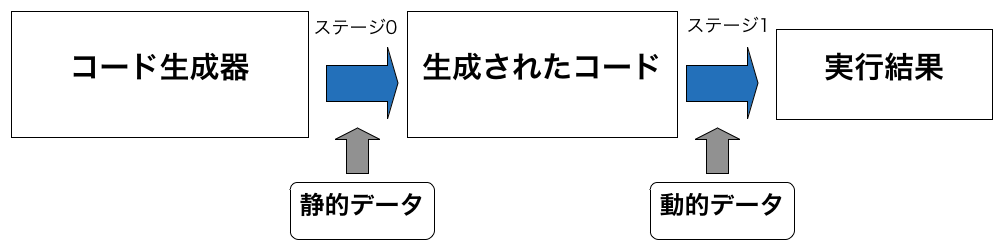
\includegraphics[clip,width=12cm]{./img/prggen.png}

  \begin{itemize}
  \item コード生成ステージとコード実行ステージ
  \item 「保守性・再利用性の高さ」と「実行性能の高さ」の両立
  \item[⇒] 段階的計算をサポートするプログラム言語
    % \item 生成するプログラムだけでなく,生成されたプログラムも型の整合性が静的に (生成前に) 保証される.
  \end{itemize}
\end{frame}

% \begin{frame}
%   \frametitle{コード生成言語の例 (MetaOCaml)}
%   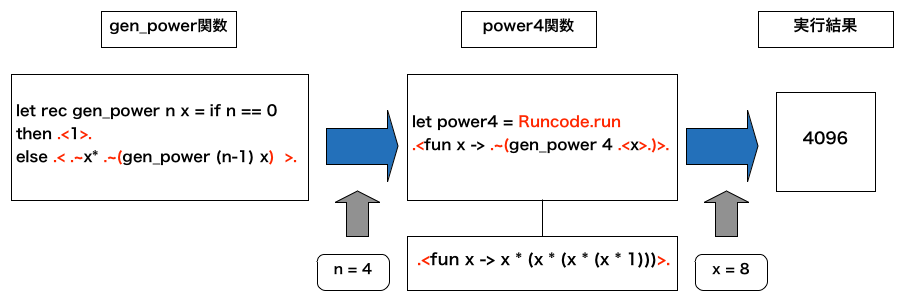
\includegraphics[clip,width=12cm]{./img/gen_power.png}
% \end{frame}

% \begin{frame}[fragile]
%   \frametitle{コード生成の例}
%   絵で説明する

%   \lstinline|@b{power : int -> int -> int}@|
% \begin{lstlisting}
% let rec power n x =
% if n == 0 then 1
% else x * power (n-1) x
% \end{lstlisting}
%   \pause
%   \lstinline|@b{gen_power : int -> int code -> int code}@|
% \begin{lstlisting}
% let rec gen_power n x =
% if n == 0 then .<1>.
% else .< .~x * .~(gen_power (n-1) x)  >.
% \end{lstlisting}
% \end{frame}

% \begin{frame}[fragile]
%   \frametitle{コード生成の例}
%   \lstinline|@b{gen_power : int -> int code -> int code}@|
% \begin{lstlisting}
% let rec gen_power n x =
% if n == 0 then .<1>.
% else .< .~x * .~(gen_power (n-1) x)  >.
% \end{lstlisting}
%   \pause
%   %   x^n の n に特化したプログラム(マルチステージングプログラミング)
%   \lstinline|@b{power4_code : (int -> int) code}@|
%   \lstinline|@b{= .<fun x_1  -> x_1 * (x_1 * (x_1 * (x_1 * 1)))>.}@|
% \begin{lstlisting}
% let power4_code = .<fun x -> .~(gen_power 4 .<x>.)>.
% \end{lstlisting}
%   \pause
%   \lstinline|@b{power4 : int -> int}@|
% \begin{lstlisting}
% let power4 = Runcode.run power4_code
% \end{lstlisting}
% \end{frame}

\subsection{効率の良いコードの生成例}

\begin{frame}[fragile]
  \frametitle{例1: 行列の積}
  $n \times n$行列の積: \lstinline|C = A B|
\begin{lstlisting}
for i = 1 to n
  for k = 1 to n
    for j = 1 to n
      c[i][j] += a[i][k] * b[k][j]
\end{lstlisting}
  \pause
  ループの展開:
\begin{lstlisting}
for i = 1 to n
  for k = 1 to n
    for j = 1 to n @r{step 4}@
      c[i][j  ] += a[i][k] * b[k][j  ]
      c[i][j@r{+1}@] += a[i][k] * b[k][j@r{+1}@]
      c[i][j@r{+2}@] += a[i][k] * b[k][j@r{+2}@]
      c[i][j@r{+3}@] += a[i][k] * b[k][j@r{+3}@]
\end{lstlisting}
\end{frame}

\begin{frame}[fragile]
  \frametitle{共通項のくくり出し}
\begin{lstlisting}
for i = 1 to n
  for k = 1 to n
    for j = 1 to n step 4
      c[i][j  ] += @r{a[i][k]}@ * b[k][j  ]
      c[i][j+1] += @r{a[i][k]}@ * b[k][j+1]
      c[i][j+2] += @r{a[i][k]}@ * b[k][j+2]
      c[i][j+3] += @r{a[i][k]}@ * b[k][j+3]
\end{lstlisting}
  \pause
\begin{lstlisting}
for i = 1 to n
  for k = 1 to n
    @r{let t = a[i][k] in}@
    for j = 1 to n step 4
      c[i][j  ] += @r{t}@ * b[k][j  ]
      c[i][j+1] += @r{t}@ * b[k][j+1]
      c[i][j+2] += @r{t}@ * b[k][j+2]
      c[i][j+3] += @r{t}@ * b[k][j+3]
\end{lstlisting}
\end{frame}

\begin{frame}[fragile]
  \frametitle{let挿入 [Danvy 1996]}

  \begin{onlyenv}<1>
    \begin{exampleblock}{let挿入}
\begin{lstlisting}
for i = 1 to n
  for k = 1 to n
    @r{let t = a[i][k] in}@
    for j = 1 to n step 4
      c[i][j  ] += @r{t}@ * b[k][j  ]
      c[i][j+1] += @r{t}@ * b[k][j+1]
      c[i][j+2] += @r{t}@ * b[k][j+2]
      c[i][j+3] += @r{t}@ * b[k][j+3]
\end{lstlisting}
    \end{exampleblock}
  \end{onlyenv}

  \begin{onlyenv}<2>
    \begin{exampleblock}{誤りのあるlet挿入}
\begin{lstlisting}
for i = 1 to n
  @r{let t = a[i][k] in}@       --- k is not bound
  for k = 1 to n in
    for j = 1 to n step 4
      c[i][j  ] += @r{t}@ * b[k][j  ]
      c[i][j+1] += @r{t}@ * b[k][j+1]
      c[i][j+2] += @r{t}@ * b[k][j+2]
      c[i][j+3] += @r{t}@ * b[k][j+3]
\end{lstlisting}
    \end{exampleblock}
  \end{onlyenv}
\end{frame}

% \begin{frame}[fragile]
%   \frametitle{共通項のくくりだし}
%   \begin{onlyenv}<1>
% \begin{lstlisting}
% for i = 1 to n
% for k = 1 to n
% for j = 1 to n step 4
% c$_{ij}$   += @r{a$_{ik}$}@ * b$_{kj}$
% c$_{i(j+1)}$ += @r{a$_{ik}$}@ * b$_{k(j+1)}$
% c$_{i(j+2)}$ += @r{a$_{ik}$}@ * b$_{k(j+2)}$
% c$_{i(j+3)}$ += @r{a$_{ik}$}@ * b$_{k(j+3)}$
% \end{lstlisting}
%   \end{onlyenv}

%   \begin{onlyenv}<2->
% \begin{lstlisting}
% for i = 1 to n
% for k = 1 to n
% @r{let t = a$_{ik}$}@
% for j = 1 to n step 4
% c$_{ij}$   += @r{t}@ * b$_{kj}$
% c$_{i(j+1)}$ += @r{t}@ * b$_{k(j+1)}$
% c$_{i(j+2)}$ += @r{t}@ * b$_{k(j+2)}$
% c$_{i(j+3)}$ += @r{t}@ * b$_{k(j+3)}$
% \end{lstlisting}
%   \end{onlyenv}
%   \begin{exampleblock}{let-insertion}<3->
%     コード生成時に,共通項をある場所へ挿入する
%   \end{exampleblock}

% \end{frame}

\begin{frame}[fragile]
  \frametitle{例2: モジュラーな配列アクセス}
\begin{lstlisting}
let main a i =
  sort a;     -- some complex computation
  access a i;
  access a i+2;

let access a i =
  @r{assert (1 <= i && i <= length a);}@
  a[i];
\end{lstlisting}
  % assert false の計算は異常終了 ⇒ 条件の成立を確認
  \lstinline|assert e|は\lstinline|e| の条件をチェック $\Rightarrow$ 適切なエラー処理をする. % assert はデバッグのための機構.assert expr という式は expr が true の時 () を返し,false の時例外 Assert_failure を発生します.Assert_failure には引数としてソースファイル名と expr の位置が指定されています.

  \pause
  main関数を展開すると・・・

  % \begin{onlyenv}<2>
% \begin{lstlisting}
% let main a i =
%   sort a;     -- some complex computation
%   access a i;
% \end{lstlisting}
%   \end{onlyenv}

  \begin{onlyenv}<3>
\begin{lstlisting}
let main a i =
  sort a;     -- some complex computation
  @r{assert (1 <= i && i <= length a);}@
  a[i];
  @r{assert (1 <= i+2 && i+2 <= length a);}@
  a[i+2];
\end{lstlisting}
  \end{onlyenv}

\end{frame}

\begin{frame}[fragile]
  \frametitle{例2: assert挿入}
\begin{lstlisting}
let main a i =
  sort a;     -- some complex computation
  @r{assert (1 <= i && i <= length a);}@
  a[i];
  @r{assert (1 <= i+2 && i+2 <= length a);}@
  a[i+2];
\end{lstlisting}
  \pause
  時間のかかる計算(sort )の前に境界チェックを行いたい.
\begin{lstlisting}
let main a i =
  @r{assert (1 <= i+2 && i+2 <= length a);}@
  @r{assert (1 <= i && i <= length a);}@
  sort a;     -- some complex computation
  a[i];
\end{lstlisting}

\end{frame}

\begin{frame}[fragile]
  \frametitle{例3: 深いネストでのassert挿入}

\begin{lstlisting}
for j = 1 to n
  for k = 1 to n
    c[j][k] := (access a j) * (access b k)
\end{lstlisting}
  \pause
  異なる地点へ,assertを挿入したい.
\begin{lstlisting}
for j = 1 to n
  @r{assert (1 <= j && j <= length a);}@
    for k = 1 to n
      @r{assert (1 <= k && k <= length b);}@
      c[j][k] := a[j] * b[k]
\end{lstlisting}

\end{frame}

\begin{frame}[fragile]
  \frametitle{安全性の静的保証}
\begin{lstlisting}
C = A B
\end{lstlisting}
  \begin{center}
    $\Downarrow$:コード生成 (コード変換,最適化を含む)
  \end{center}
\begin{lstlisting}
for i = 1 to n
  for k = 1 to n
    @r{let t = a[i][k]}@
    for j = 1 to n step 4
      c[i][j  ] += @r{t}@ * b[k][j]
      c[i][j+1] += @r{t}@ * b[k][j+1]
      c[i][j+2] += @r{t}@ * b[k][j+2]
      c[i][j+3] += @r{t}@ * b[k][j+3]
\end{lstlisting}

  \begin{exampleblock}{安全性の静的保証}
    動的に生成されたコードのデバッグは困難\\
    ⇒ コード生成の前に安全性を保証したい
  \end{exampleblock}

\end{frame}

\subsection{段階的計算の課題}

\begin{frame}
  \frametitle{コード生成における課題}
  % もっとコンパクトに
  生成されたコードの信頼性(正しさ)
  \begin{itemize}
  \item パラメータに応じて,非常に多数のコードが生成される
    % \item 構文的,意味的に正しくないプログラムを生成しやすい
  \item 生成したコードのデバッグが容易ではない
  \end{itemize}

  \uncover<2->{従来研究}
  \begin{itemize}
  \item<2-> コード生成プログラムが,安全なコードのみを生成する事を保証
    % \item<2-> 安全なコード: 構文,型,変数束縛が正しいプログラム
    %%% \item<2-> let挿入等を実現する\alert{計算エフェクトを含む場合の安全性保証の研究は未整備}
  \item<2-> let挿入等を実現する\alert{計算エフェクトを含む場合の安全性保証は研究途上}
  \end{itemize}
\end{frame}

\section{研究の目的}
% s0/r0 にフォーカスした話をする.
\begin{frame}
  \frametitle{研究の目的}
  %%% 従来研究の階層化shift/resetやマルチプロンプトshift/resetは比較的複雑な理論で安全性を確保していたのだが,よりシンプルな理論体系で安全性を実現したい.
  %%%
  %%% そこで,従来よりもシンプルなshift0/reset0に着目して,多段階のlet挿入を行うようなコード生成を行う
  %%%
  %%% \begin{itemize}
  %%% \item コード生成に必要な種々の計算エフェクトが,安全に正しく使われているかを自動的に検査
  %%% \item 計算エフェクトとして,特に,shift0/reset0 によるコントロールオペレータを用いたコード生成
  %%% \end{itemize}
  %%%
  %%% \pause
  %%% 研究項目
  %%% \begin{itemize}
  %%% \item shift0/reset0 を持つプログラム生成のための体系の構築
  %%% \item shift0/reset0 を持つプログラム生成のための言語の設計と実装
  %%% \end{itemize}

  \begin{block}{\textbf{表現力}と\textbf{安全性}を兼ね備えたコード生成言語の構築}
    \begin{itemize}
    \item 表現力: 多段階let挿入,メモ化等の技法を表現
    \item 安全性: 生成されるコードの一定の性質を静的に検査
    \end{itemize}
  \end{block}

  \medskip
  \pause

  \begin{block}{本研究: より簡潔でより強力なコントロールオペレータに基づくコード生成体系の構築}

    \begin{itemize}
    \item コントロールオペレータ shift0/reset0 を利用
    \item 種々のコード生成技法を表現
    \item 型システムを構築して型安全性を保証
    \end{itemize}
  \end{block}


\end{frame}

% \section{型システム}

\section{研究の内容}

% \begin{frame}
%   \frametitle{型システム}

%   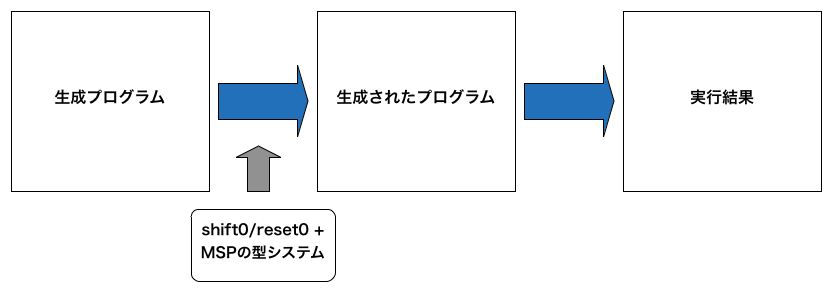
\includegraphics[clip,width=12cm]{./img/type_system0.png}

%%%   従来研究のマルチプロンプト等の複雑な型システムよりも簡単なもので,同様な安全性を実現したい.

%   \begin{itemize}
%   \item MSPでの型システムの健全性とは,プログラム生成前に,型検査に通っていれば,生成後のコードに型エラーは絶対に起きないようなシステムである.
%   \end{itemize}
%   型システムとは,実行前のコンパイルの時点で,データの使われ方を検査することで,一貫性を保証し,信頼性の向上につながるものです
%   また,多相型を用いることで,1つのプログラムをさまざまな型のデータに使用することができ,生産性を高めることができます.

% \end{frame}

\subsection{コントロールオペレータ}

\begin{frame}
  \frametitle{コントロールオペレータ}

  % shift0/reset0 の立ち位置の説明
  % コントロールオペレータとしてこの様なものがあるが,本研究では,その中でもあまり研究されていない比較的新しいここ五年ほどで出てきたshift0/reset0を用いる.
  % shift0/reset0 は shift/resetとほとんど同じ計算規則なのにむしろ簡単な程度だが,表現力が非常に強い
  % より簡潔なCPSの意味論でより強い表現力を持つ


  % より簡潔なCPSの意味論をもち,
  % それでいて,表現力は階層的shift/resetを完全に表現できる.(例えば多段階let挿入が可能)
  % ごく最近2011年以降研究されている.
  \begin{block}{プログラミング言語におけるプログラムを制御するプリミティブ}
    \begin{itemize}
    \item exception (例外): % C++, Java, ML
    \item call/cc (第一級継続): % Scheme, SML/NJ
    \item shift/reset (限定継続): % Racket, Scala, OCaml
      \begin{itemize}
      \item 1989年以降多数研究がある
      \item コード生成におけるlet挿入が実現可能
        % \item shift/reset + コード生成の型システムが幾つか提案されている
      \end{itemize}
    \item \alert{shift0/reset0}
      \begin{itemize}
        \item 2011年以降研究が活発化.
        \item コード生成における多段階let挿入が可能
      \end{itemize}
    \end{itemize}
  \end{block}
\end{frame}


\begin{frame}[fragile]
  \frametitle{関数型言語のプログラム例}
  \begin{onlyenv}<1>
\begin{lstlisting}
(3 + 5 + k(7))
\end{lstlisting}
  \end{onlyenv}
  \pause

  \begin{onlyenv}<2>
\begin{lstlisting}
(3 + 5 + k(7)) = (3 + 5 + k 7)
\end{lstlisting}
  \end{onlyenv}
  \pause

  \begin{onlyenv}<3>
\begin{lstlisting}
(3 + 5 + k(7))
@r{reset0}@ (3 + 5 + k(7))
\end{lstlisting}
  \end{onlyenv}
  \pause

  \begin{onlyenv}<4>
\begin{lstlisting}
(3 + 5 + k(7))
@r{reset0}@ (3 + 5 + k(7)) $\Rightarrow$ (3 + 5 + k(7))
\end{lstlisting}
  \end{onlyenv}
  \pause

  \begin{onlyenv}<5>
\begin{lstlisting}
(3 + 5 + k(7))
@r{reset0}@ (3 + 5 + k(7)) $\Rightarrow$ (3 + 5 + k(7))
@r{reset0}@ (3 + (@r{shift0}@ k -> 5 + k(7))) $\Rightarrow$ ...
\end{lstlisting}
  \end{onlyenv}

\end{frame}

\begin{frame}[fragile]
  \frametitle{コントロールオペレータshift0/reset0}
  % 実際のコードによる説明
  % reset0 とshift0の間に挟まれた文脈(プログラム)の一部を切り取って他に貼り付ける機能があります.
  \begin{onlyenv}<1>
\begin{lstlisting}
  @r{reset0}@ (3 + (@r{shift0}@ k -> 5 + k(7)))

\end{lstlisting}
  \end{onlyenv}

  \begin{onlyenv}<2>
\begin{lstlisting}
  @r{reset0}@ (3 + (@r{shift0}@ k -> @g{5 + k(7)}@))
$\Rightarrow$ @g{(5 + k(7))}@

\end{lstlisting}
  \end{onlyenv}

  \begin{onlyenv}<3>
\begin{lstlisting}
  @r{reset0}@ @g{(3 +}@ (@r{shift0}@ k -> 5 + k(7))@g{)}@
$\Rightarrow$ (5 + k(7)) where k = @r{reset0}@ @g{(3 + [])}@

\end{lstlisting}
  \end{onlyenv}

  \begin{onlyenv}<4>
\begin{lstlisting}
  @r{reset0}@ (3 + (@r{shift0}@ k -> 5 + k(7)))
$\Rightarrow$ (5 + k(7)) where k = @r{reset0}@ (3 + [])
$\Rightarrow$ (5 + @r{reset0}@ (3 + 7)) $\Rightarrow$  15
\end{lstlisting}
  \end{onlyenv}


\end{frame}



\begin{frame}[fragile]
  \frametitle{shift0/reset0 によるlet挿入}
  % 実際のコードによる説明
  % 前述のようなことができるので,
  % このshift0はreset0までのプログラムの部分を切り取って,他の部分に貼り付けるという効果があります.で,この計算はこのようになりますが,ここで注目していただきたいのはshift0というのは外側のプログラムを操作する機能があるということです.
  % 先ほどコード生成の例でお話したlet挿入がshift0/reset0で行えるということをお話します.さきほどと同じような例ですが,今回はshift0の本体にlet x = 5 in というプログラムが入っています.これを先ほどと同じように実行してみると,今度は外側の文脈(プログラムの一部)を切り取り,k のところに貼り付けます.するとこのようにプログラムが実行されます.
  % これは見方を変えると,外側を切り取って中に入れたというよりは,letが外側に出たというふうに見ることもできます.
  % このように外側を切り取るコントロールオペレータ (shift0/reset0) を使うとlet挿入が実現できることがわかると思います.

  % 余談: このコードで問題なのは,コード生成におけるlet挿入ではなく,今すぐ動いてしまうletを動かしているだけで,こういう例は本当はlet挿入とは言わない...らしい
  \begin{onlyenv}<1>
\begin{lstlisting}
  @r{reset0}@ (3 + (@r{shift0}@ k -> let x = 5 in k(x)))
\end{lstlisting}
  \end{onlyenv}

  \begin{onlyenv}<2>
\begin{lstlisting}
  @r{reset0}@ (3 + (@r{shift0}@ k -> @g{let x = 5 in k(x)}@))
$\Rightarrow$ @g{(let x = 5 in k(x))}@
\end{lstlisting}
  \end{onlyenv}

  \begin{onlyenv}<3>
\begin{lstlisting}
  @r{reset0}@ @g{(3 +}@ (@r{shift0}@ k -> let x = 5 in k(x))@g{)}@
$\Rightarrow$ (let x = 5 in k(x))
           where k = @r{reset0}@ @g{(3 + [])}@

\end{lstlisting}
  \end{onlyenv}

  \begin{onlyenv}<4>
\begin{lstlisting}
  @r{reset0}@ (3 + (@r{shift0}@ k -> let x = 5 in k(x)))
$\Rightarrow$ (let x = 5 in k(x))
           where k = @r{reset0}@ (3 + [])
$\Rightarrow$ (let x = 5 in @r{reset0}@ (3 + x))
\end{lstlisting}
  \end{onlyenv}


\end{frame}

% \begin{frame}[fragile]
%   \frametitle{shift0/reset0とshift/reset の比較 }
%   %   実際のコードによる説明
%   shift/reset では多段階let-insertion はfailする.しかし,shift0/reset0では成功するということを例で書きたい.そのために,letを含んだ例を書く.
% \begin{lstlisting}
% @b{reset0}@ (10 * @r{reset0}@ (3 +
% (@r{shift0}@ k1 -> @b{shift0}@ k2 -> 5 + k1(k2(7)))))
% $\Rightarrow$ @b{reset0}@ (10 * @b{shift0}@ k2 -> 5 + k1(k2(7)))
% $\Rightarrow$ 5 + k1(k2(7)) where k1 = @r{reset0}@(3+[]),
% k2 = @b{reset0}@(10*[])
% $\Rightarrow$ 78
% \end{lstlisting}
%   \pause
%   この例を shift/reset にすると・・・
% \begin{lstlisting}
% @b{reset}@ (10 * @r{reset}@ (3 +
% (@r{shift}@ k1 -> @b{shift}@ k2 -> 5 + k1(k2(7)))))
% $\Rightarrow$ @b{reset}@ (10 * @r{reset}@(@b{shift}@ k2 -> 5 + k1(k2(7))))
% $\Rightarrow$ @b{reset}@ (10 * @r{reset}@(5 + k1(k2(7))))
% where k1 = @r{reset}@(3+[]),
% k2 = @b{reset}@([])
% $\Rightarrow$ 150
% \end{lstlisting}

% \end{frame}

\begin{frame}[fragile]
  \frametitle{shift0/reset0による多段階let挿入}
  % 実際のコードによる説明
  % assert insertion の例を書く
  % ...の部分を埋める.
  % コードが複雑なので詳細には説明しないが,shift0/reset0はこのように動作し,異なる地点(多段階の)にassertを挿入したり,letを挿入することが実現できる.

  % ここで,\lstinline|access|とは,以下の様な関数である.配列 a の要素外にアクセスしようとすると,assert により,Assert_failure を発生し,その発生した場所を出力する.


\begin{lstlisting}
for j = 1 to n
  for k = 1 to n
    c[j][k] := (access a j) * (access b k)
\end{lstlisting}
  \pause
  $\Rightarrow$

\begin{lstlisting}
for j = 1 to n
  @r{assert (1 <= j && j <= length a);}@
  for k = 1 to n
    @b{assert (1 <= k && k <= length b);}@
    c[j][k] := a[j] * b[k]
\end{lstlisting}
  \pause
\begin{lstlisting}
for j = 1 to n
  @r{reset0}@(
  for k = 1 to n
    @b{reset0}@(
    c[j][k] := (@r{access2}@ a j) * (@b{access1}@ b k)))
\end{lstlisting}
\end{frame}

\begin{frame}[fragile]
  \frametitle{shift0/reset0による多段階let挿入}

\begin{lstlisting}
for j = 1 to n  @m{reset0(}@
  @m{for k = 1 to n}@  @g{reset0(}@
    @g{c[j][k] :=}@ (@r{access2}@ a j) @g{* (access1 b k))}@@m{)}@
\end{lstlisting}

  \pause

\begin{lstlisting}
let @r{access2}@ a j =
  @g{shift0 k1}@ -> @m{shift0 k2}@ ->
       assert (1 <= j && j <= length a);
       @m{k2}@ (@g{k1}@ (a[j]))
\end{lstlisting}

  \pause

\begin{lstlisting}
@g{k1 = reset0( c[j][k] := [ ] * (access1 b k) )}@
@m{k2 = reset0( for k = 1 to n [ ] )}@
\end{lstlisting}
\end{frame}

\begin{frame}[fragile]
  \frametitle{shift0/reset0による多段階let挿入}

\begin{lstlisting}
for j = 1 to n  @m{reset0(}@
  @m{for k = 1 to n}@  @g{reset0(}@
    @g{c[j][k] :=}@ (@r{access2}@ a j) @g{* (access1 b k))}@@m{)}@
\end{lstlisting}

  \pause
$\Rightarrow$

\begin{lstlisting}
for j = 1 to n
  assert (1 <= j && j <= length a);
    @m{k2}@ (@g{k1}@ (a[j]))
\end{lstlisting}

  \pause
$\Rightarrow$

\begin{lstlisting}
for j = 1 to n
  @r{assert (1 <= j && j <= length a);}@
    for k = 1 to n
      c[j][k]:=[] * (access1 b k)
\end{lstlisting}

\end{frame}

\begin{frame}[fragile]
  \frametitle{shift0/reset0とshift/reset}
  % shift0/reset0はshift/reset とほぼ同様な計算規則で定義されている.その差は僅かです
  % しかし shiftは直近のresetまでのプログラムの部分を切り取ることができますが,それ以上の2番目3番目のresetまでのプログラムの部分を切り取ることはできません.
  % 一方でMaterzokらによってshift0をうまく使うことによって直近のshift0だけでなく,2番目3番目のreset0までのプログラムの部分を切り取ることができることがわかっています.

% このような働きを持つオペレータはコード生成に非常に有用であることに着目してこの研究をはじめました.Materzokらはラムダ計算に対してshift0/reset0の性質を解明したのですが,本研究ではこれをコード生成言語の多段階let挿入に使えることを思いつき,そのような体系を作りたいというのが本研究の基本着想です.

  shift0/reset0とshift/resetはわずかに異なる

% より簡潔なCPSの意味論をもち,
  % それでいて,表現力は階層的shift/resetを完全に表現できる.(例えば多段階let挿入が可能)
  % ごく最近2011年以降研究されている.
  \begin{center}
    shift0/reset0: $\langle K [S_0 f.e] \rangle \rightsquigarrow e \{ f / \lambda x . \langle K [x] \rangle \}$\\
    shift/reset:  \,\,\,\,$\langle K [S f.e] \rangle \rightsquigarrow \langle e \{ f / \lambda x . \langle K [x] \rangle \} \rangle $
  \end{center}

  % shift0は,直近のreset0より,遠くのreset0までアクセスできる.
  \begin{columns}
    \begin{column}{.5\textwidth}
      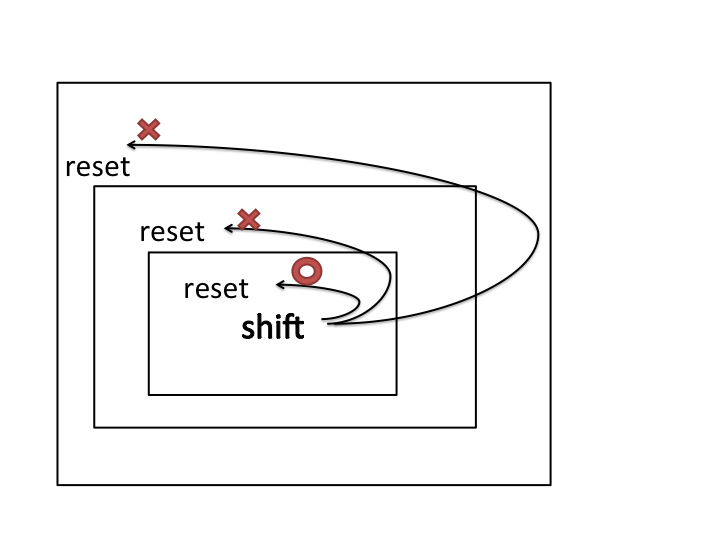
\includegraphics[clip,width=8cm]{./img/sr.png}
    \end{column}

    \begin{column}{.5\textwidth}
      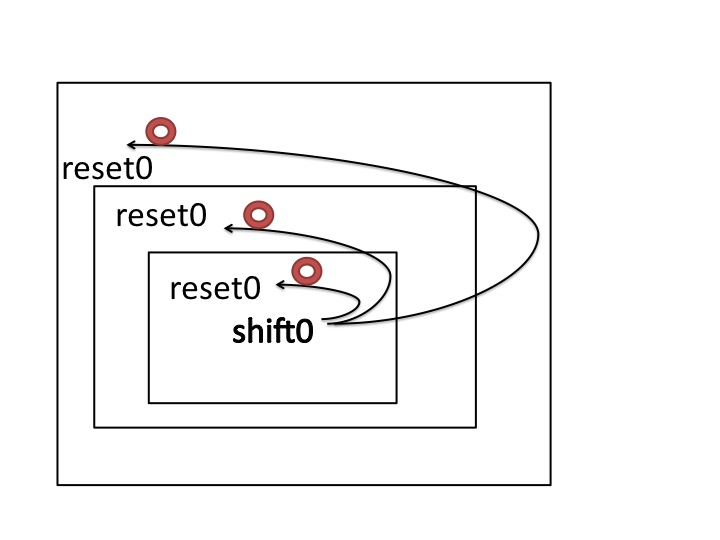
\includegraphics[clip,width=8cm]{./img/s0r0.png}
    \end{column}
  \end{columns}

  % \begin{itemize}
  % \item 「1つ上」のスコープまでのジャンプ ... shift/reset で実現可能
  % \item 「n個上」のスコープまでのジャンプ ... shift0/reset0 で実現可能
  % \end{itemize}

\end{frame}

\subsection{本研究の着想}
\begin{frame}
  \frametitle{本研究の着想}
  \begin{itemize}
  \item shift/resetでは,多段階のlet挿入は実現できない $\Rightarrow$ shift0/reset0では実現可能
  \item 階層化shift/resetでは実現可能 $\Rightarrow$ 型システムが複雑,シンプルな意味論がない
  \end{itemize}

  \pause
  shift0/reset0は単純なCPS変換,CPS意味論をもち,多段階let挿入が実現できるところに着目$\Rightarrow$ コード生成への応用

  % 本研究は単一のshift0/reset0で単純なCPS変換,CPS意味論を持つオペレータで多段階let挿入が実現できるところに着目して,これをコード生成に使おうというのが本研究の着想である.
  % optional:
  % 従来研究でもマルチプロンプトや階層化shift/resetでは実現できるのだが,これやあれがあって,型システムがふくざつになったりする.シンプルな意味論がない...

\end{frame}


% \section{本研究の手法}

% \begin{frame}
%   \frametitle{本研究の手法}
%%   ここは本研究でめざす型システムのスライドで説明する.

%   目的:
%   \begin{itemize}
%   \item shift0/reset0 を持つコード生成言語の型システムの設計
%   \item 深く入れ子になった内側からの,let挿入,assertion挿入の
%     関数プログラミング的実現
%   \end{itemize}

%   \pause
%   困難・問題点
%   \begin{itemize}
%   \item shift0/reset0 は shift/resetより強力であるため,型システムが非常に複雑
%   \item コード生成言語の型システムも一定の複雑さ
%   \item ⇒ 単純な融合は困難
%   \end{itemize}

%   \pause
%   本研究の手法
%   \begin{itemize}
%   \item shift0/reset0 の型システムを単純化; let挿入等に絞る
%   \item これをコード生成言語の型システムに融合
%   \item 型システムの安全性を保証: Kameyama+ 2009, Sudo+2014 の手法を利用
%   \end{itemize}

% \end{frame}

\begin{frame}
  \frametitle{型システム}

  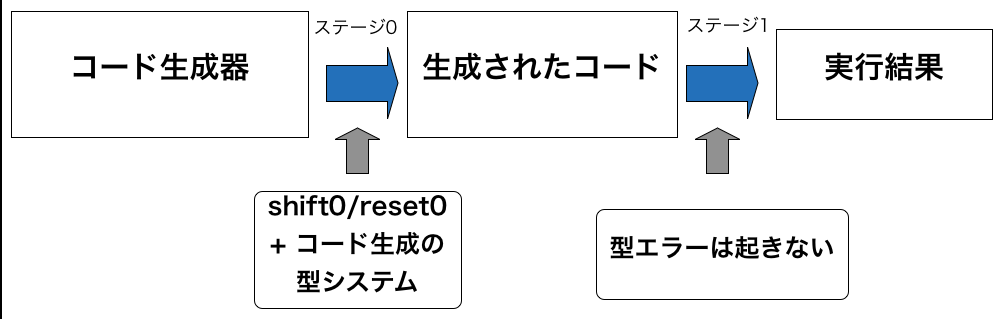
\includegraphics[clip,width=12cm]{./img/type_system1.png}

  % 従来研究のマルチプロンプト等の複雑な型システムよりも簡単なもので,同様な安全性を実現したい.

  \begin{itemize}
  \item MSPでの型システムの健全性とは,プログラム生成前に,型検査に通っていれば,生成後のコードに型エラーは絶対に起きないようなシステムである.
  \item 計算エフェクト(コントロールオペレータ)などがあるコード生成言語の型安全性は難しい課題であり多数の研究がある.
  \end{itemize}
  % 型システムとは,実行前のコンパイルの時点で,データの使われ方を検査することで,一貫性を保証し,信頼性の向上につながるものです
  % また,多相型を用いることで,1つのプログラムをさまざまな型のデータに使用することができ,生産性を高めることができます.

  % 型安全性やスコープ安全性も保証される.

\end{frame}


\begin{frame}[fragile]
  \frametitle{研究項目}
\begin{enumerate}
\item shift0/reset0 を持つプログラム生成のための体系の構築
  \begin{itemize}
  \item 型システムと操作的意味論の構築
  \item 型の健全性の証明
  \end{itemize}
\item shift0/reset0 を持つプログラム生成のための言語の設計と実装
  \begin{itemize}
  \item 抽象機械による実装
  \item 効率のよいコード生成プログラムの例の作成
  \end{itemize}
\end{enumerate}

\end{frame}

\begin{frame}[fragile]
  \frametitle{本研究の手法}
  % 実際に信頼性の高いコード生成言語とshift0/reset0をもつ言語を融合するために以下の様な物を考えたい.
  \begin{columns}

    \begin{column}{1.\textwidth}%% [横幅] 0.2\textwidth = ページ幅の 20 %
      \center
      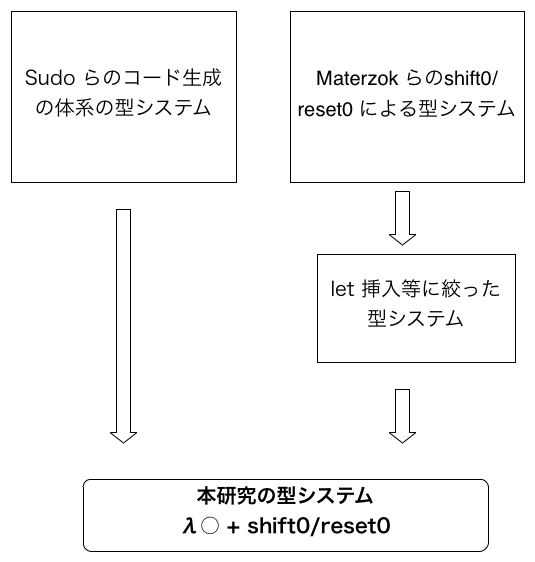
\includegraphics[clip,height=7cm]{./img/type_system_me.png}
    \end{column}

    % \begin{column}{0.4\textwidth}%% [横幅] 0.2\textwidth = ページ幅の 20 %
    %   \begin{itemize}
    %   \item
    %   \item
    %   \item
    %   \end{itemize}
    % \end{column}

    % \begin{column}{0.4\textwidth}%% [横幅] 0.2\textwidth = ページ幅の 20 %
    %   \begin{itemize}
    %   \item Sudoらの段階的計算の型システム $\lambda \circ _{\leq}$
    %   \item[] $+$
    %   \item Materzokらのコントロールオペレータshift0/reset0 を持つ体系の型システム$\lambda ^{S0}_{\leq}$のサブセット
    %   \end{itemize}
    % \end{column}

  \end{columns}
\end{frame}

% \begin{frame}[fragile]
%   \frametitle{shift0/reset0のインタプリタ}
%   % 現在のところ,このような設計をして,実例について学んだ後,shift0/reset0のインタプリタを作ってみました.
% \begin{lstlisting}
% type term = Var of string
%           | Abs of string * term
%           | App of term * term
%           | Shift0 of term
%           | Reset0 of term

% type value = VAbs of ((value * c) -> value)
% | VCont of cont

% and cont = (v -> v)
% \end{lstlisting}


%   % 今まで出てきた例がきちんと動くよねーというような
%   % インタプリタの実行例を見せて,頑張った感を魅せるだけのスライド

% \begin{itemize}
% \item 型のないshift0/reset0 を持つ体系の言語のインタプリタを実装した.
% \end{itemize}

% \end{frame}


\section{まとめと今後}

\begin{frame}
  \frametitle{まとめと今後}
  \begin{itemize}
  \item 多段階let挿入がshift0/reset0で記述可能なことを見た.
  \item[] shift0/reset0を導入した言語を考えると従来より,簡潔で,検証しやすい体系ができるということを提案した.
  % \item その一歩として,型のないshift0/reset0 を入れた体系である$\lambda ^{S0}$のインタプリタを実装した.
  \item Sudoらのコード生成言語の型システムを利用し,shift0/reset0を組み込んだ体系について検討中である.
  \item 今後,型システムの設計を完成させ健全性の証明を行う.% 型検査器等の実装行う
  \end{itemize}
\end{frame}


%% ===============================================
%% 予備スライド
%% ===============================================

%% 予備スライドは appendix 環境の中に書きましょう.
\begin{appendix}

  %% 予備スライドの先頭に APPENDIX と書かれたページを挟む(お好みで消去しても良い)
  \frame[plain]{\centerline{\Huge\bfseries\color{structure}APPENDIX}}

  \section{コード生成言語}
  \subsection{安全性}

\begin{frame}[fragile]
  \frametitle{コード生成言語の安全性}
\begin{lstlisting}
let rec power n x =
  if n = 0 then 1
  else x * power (n-1) x
in power 3 2                 ==> 8
\end{lstlisting}
\begin{lstlisting}
let rec gen_power n x =
  if n = 0 then <1>
  else < ~x * ~(gen_power (n-1) x)>
in gen_power 3 <2>           ==> <2 * 2 * 2>
\end{lstlisting}
\begin{lstlisting}
let rec @b{wrong}@ n x =
  if n = 0 then <1>
  else < ~x @b{&&}@ ~(wrong (n-1) x)>  ==> error
\end{lstlisting}
  \texttt{(wrong 3 <2>)} を実行することはない.
\end{frame}

\subsection{型システム}

\begin{frame}[fragile]
  \frametitle{コード生成言語の型システム}
\begin{lstlisting}
let rec power n x =
  if n = 0 then 1
  else x * power (n-1) x
==> power : int -> int -> int
\end{lstlisting}
\begin{lstlisting}
let cde = < 3 + 5>
==> cde : int code
\end{lstlisting}
\begin{lstlisting}
let f x = < ~x + 7>
==> f : int code -> int code
\end{lstlisting}
\begin{lstlisting}
let rec gen_power n x =
  if n = 0 then <1>
  else < ~x * ~(gen_power (n-1) x)>
==> gen_power : int -> int code -> int code
\end{lstlisting}

  生成されたコードの内部の型付けも行われる.
\end{frame}

\section{本研究の型システム}

\begin{frame}[fragile]
  \frametitle{本研究の型システム(1)}

  1. Sudoらの型システムのアイディアを利用:
  変数スコープを表す変数a1,a2,...を使って,
  型の中で変数スコープを表す.

\begin{lstlisting}
let f x = < ~x + 7>
==> f : int code@r{^a1}@ -> int code@r{^a1}@
\end{lstlisting}
\begin{lstlisting}
let g = <fun y -> y + 7>
==> g : (int -> int) code@r{^a2}@
\end{lstlisting}
\begin{lstlisting}
let h = fun x -> <fun y -> ~x + y>
==> h : int code @r{^a1}@ -> (int -> int) code@r{^a2}@
    where @r{a2 < a1}@
\end{lstlisting}

  変数スコープの包含関係を,変数a1,a2...に対する順序で表現
\end{frame}

\begin{frame}[fragile]
  \frametitle{本研究の型システム(2)}

  2. let挿入において shift0/reset0 が型安全性を保つ条件を見つける

\begin{lstlisting}
... (reset0 ( ... (shift0 k -> ... (k  ...))))
 a0           a1                a2     a3
\end{lstlisting}

  \medskip

  let挿入: a2 にある letを reset0 の場所へ移動する.

  \medskip
  ⇒ a1 と a2 の場所を交換しても,型エラーが起きない条件を同定し,
  その条件のもとで,型安全性を証明すればよい.

  \medskip
  ⇒ a1 で生成される変数は a2 で使えないよう,条件を付ければよい.

\end{frame}

\begin{frame}[fragile]
  \frametitle{本研究の型システム(3)}

  3. 型安全性(型システムの健全性; Subject Reduction等の性質)を厳密に証明する.

  \begin{block}{Subject Redcution Property}
    $\Gamma \vdash M: \sigma$ が導ければ(プログラム$M$が型検査を通れば),
    $M$を計算して得られる任意の$N$に対して,
    $\Gamma \vdash N: \sigma$ が導ける($N$も型検査を通り,$M$と同じ型,
    同じ自由変数を持つ.)
  \end{block}

\end{frame}


  % \begin{frame}
  %   \frametitle{予備のスライド}
  %   \begin{itemize}
  %   \item 型システムって何 A. 値を特定の種類 (型)に分類し,プログラムが正しく振る舞うこと,といった性質について保証する手法.(安全性の保証)
  %   \item 単純化するとは具体的にどうするのか  A. shift0/reset0 の sub-typing 等をなくした体系を考えるかもしれない.
  %   \item 部分型付け (sub-typing)とは A.項の部分に対して型付けを行うということ.例えば...
  %   \end{itemize}

  % \end{frame}

\end{appendix}

\end{document}

%%% Local Variables:
%%% mode: latex
%%% TeX-master: t
%%% End:
